\documentclass{article}

\usepackage[utf8]{inputenc}
\usepackage{tikz}
\usepackage{amsmath}
\usepackage{mathtools}
\usepackage{amsfonts}
\usepackage{amssymb}
\usepackage{sectsty}
\usepackage{xcolor}
\usepackage[paperwidth=180mm, paperheight=290mm, left=10mm, top=10mm, bottom=10mm, right=10mm, margin=10mm]{geometry}
\usepackage{ragged2e}
\usepackage{listings}
\usepackage[hidelinks]{hyperref}

\definecolor{def}{RGB}{255, 150, 89}
\definecolor{tit}{RGB}{217, 84, 80}
\definecolor{emp}{RGB}{150, 206, 180}
\definecolor{acc}{RGB}{255, 234, 150}
\definecolor{txt}{RGB}{249, 232, 232}
\definecolor{back}{RGB}{22, 22, 22}

\sectionfont{\fontsize{20.74}{35}\ttfamily}
\subsectionfont{\color{tit}\fontsize{17.28}{17.28}\ttfamily}

\DeclareFontFamily{\encodingdefault}{\ttdefault}{
  \hyphenchar\font=\defaulthyphenchar
  \fontdimen2\font=0.33333em
  \fontdimen3\font=0.16667em
  \fontdimen4\font=0.11111em
  \fontdimen7\font=0.11111em
}

\newcommand{\R}{\mathbb{R}}
\newcommand{\N}{\mathbb{N}}
\newcommand{\Q}{\mathbb{Q}}
\newcommand{\Z}{\mathbb{Z}}
\newcommand{\C}{\mathbb{C}}
\newcommand{\cont}{\mathfrak{c}}

\geometry{a4paper, textwidth=155mm, textheight=267mm, left=15mm, top=15mm, right=15mm, marginparwidth=0mm}
\setlength\parindent{15pt}

\pagestyle{empty}

\begin{document}\pagecolor{back}\color{txt}\ttfamily
    
    1. \begin{tikzpicture}
        \node(a) at (0,0) {a};
        \node(b) at (0,1) {b};
        \node(c) at (1,1.5) {c};
        \node(d) at (2,1) {d};
        \node(f) at (1, -0.5) {f};
        \node(e) at (2, 0) {e};
        \draw(a)--(b);
        \draw(a)--(c);
        \draw(c)--(b);
        \end{tikzpicture}\\
        
        2. \begin{tikzpicture}
        \node(a) at (0,0) {a};
        \node(b) at (0,1) {b};
        \node(c) at (1,1.5) {c};
        \node(d) at (2,1) {d};
        \node(f) at (1, -0.5) {f};
        \node(e) at (2, 0) {e};
        \draw(a)--(b);
        \draw(a)--(d);
        \draw(d)--(b);
        \end{tikzpicture}\\
        
        3. 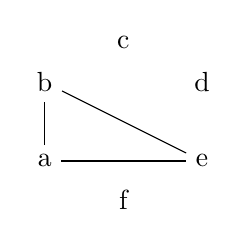
\begin{tikzpicture}
        \node(a) at (0,0) {a};
        \node(b) at (0,1) {b};
        \node(c) at (1,1.5) {c};
        \node(d) at (2,1) {d};
        \node(f) at (1, -0.5) {f};
        \node(e) at (2, 0) {e};
        \draw(a)--(b);
        \draw(a)--(e);
        \draw(e)--(b);
        \end{tikzpicture}\\
        
        4. \begin{tikzpicture}
        \node(a) at (0,0) {a};
        \node(b) at (0,1) {b};
        \node(c) at (1,1.5) {c};
        \node(d) at (2,1) {d};
        \node(f) at (1, -0.5) {f};
        \node(e) at (2, 0) {e};
        \draw(a)--(b);
        \draw(a)--(f);
        \draw(f)--(b);
        \end{tikzpicture}\\
        
        5. 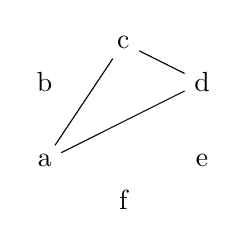
\begin{tikzpicture}
        \node(a) at (0,0) {a};
        \node(b) at (0,1) {b};
        \node(c) at (1,1.5) {c};
        \node(d) at (2,1) {d};
        \node(f) at (1, -0.5) {f};
        \node(e) at (2, 0) {e};
        \draw(a)--(c);
        \draw(a)--(d);
        \draw(d)--(c);
        \end{tikzpicture}\\
        
        6. 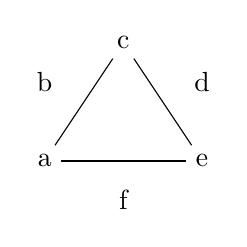
\begin{tikzpicture}
        \node(a) at (0,0) {a};
        \node(b) at (0,1) {b};
        \node(c) at (1,1.5) {c};
        \node(d) at (2,1) {d};
        \node(f) at (1, -0.5) {f};
        \node(e) at (2, 0) {e};
        \draw(a)--(c);
        \draw(a)--(e);
        \draw(e)--(c);
        \end{tikzpicture}\\
        
        7. \begin{tikzpicture}
        \node(a) at (0,0) {a};
        \node(b) at (0,1) {b};
        \node(c) at (1,1.5) {c};
        \node(d) at (2,1) {d};
        \node(f) at (1, -0.5) {f};
        \node(e) at (2, 0) {e};
        \draw(a)--(c);
        \draw(a)--(f);
        \draw(f)--(c);
        \end{tikzpicture}\\
        
        8. \begin{tikzpicture}
        \node(a) at (0,0) {a};
        \node(b) at (0,1) {b};
        \node(c) at (1,1.5) {c};
        \node(d) at (2,1) {d};
        \node(f) at (1, -0.5) {f};
        \node(e) at (2, 0) {e};
        \draw(a)--(d);
        \draw(a)--(e);
        \draw(e)--(d);
        \end{tikzpicture}\\
        
        9. 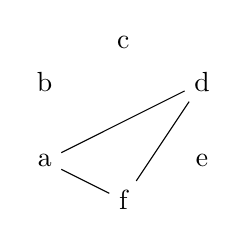
\begin{tikzpicture}
        \node(a) at (0,0) {a};
        \node(b) at (0,1) {b};
        \node(c) at (1,1.5) {c};
        \node(d) at (2,1) {d};
        \node(f) at (1, -0.5) {f};
        \node(e) at (2, 0) {e};
        \draw(a)--(d);
        \draw(a)--(f);
        \draw(f)--(d);
        \end{tikzpicture}\\
        
        10. \begin{tikzpicture}
        \node(a) at (0,0) {a};
        \node(b) at (0,1) {b};
        \node(c) at (1,1.5) {c};
        \node(d) at (2,1) {d};
        \node(f) at (1, -0.5) {f};
        \node(e) at (2, 0) {e};
        \draw(a)--(e);
        \draw(a)--(f);
        \draw(f)--(e);
        \end{tikzpicture}\\
        
        11. \begin{tikzpicture}
        \node(a) at (0,0) {a};
        \node(b) at (0,1) {b};
        \node(c) at (1,1.5) {c};
        \node(d) at (2,1) {d};
        \node(f) at (1, -0.5) {f};
        \node(e) at (2, 0) {e};
        \draw(b)--(c);
        \draw(b)--(d);
        \draw(d)--(c);
        \end{tikzpicture}\\
        
        12. 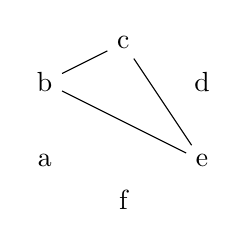
\begin{tikzpicture}
        \node(a) at (0,0) {a};
        \node(b) at (0,1) {b};
        \node(c) at (1,1.5) {c};
        \node(d) at (2,1) {d};
        \node(f) at (1, -0.5) {f};
        \node(e) at (2, 0) {e};
        \draw(b)--(c);
        \draw(b)--(e);
        \draw(e)--(c);
        \end{tikzpicture}\\
        
        13. \begin{tikzpicture}
        \node(a) at (0,0) {a};
        \node(b) at (0,1) {b};
        \node(c) at (1,1.5) {c};
        \node(d) at (2,1) {d};
        \node(f) at (1, -0.5) {f};
        \node(e) at (2, 0) {e};
        \draw(b)--(c);
        \draw(b)--(f);
        \draw(f)--(c);
        \end{tikzpicture}\\
        
        14. \begin{tikzpicture}
        \node(a) at (0,0) {a};
        \node(b) at (0,1) {b};
        \node(c) at (1,1.5) {c};
        \node(d) at (2,1) {d};
        \node(f) at (1, -0.5) {f};
        \node(e) at (2, 0) {e};
        \draw(b)--(d);
        \draw(b)--(e);
        \draw(e)--(d);
        \end{tikzpicture}\\
        
        15. \begin{tikzpicture}
        \node(a) at (0,0) {a};
        \node(b) at (0,1) {b};
        \node(c) at (1,1.5) {c};
        \node(d) at (2,1) {d};
        \node(f) at (1, -0.5) {f};
        \node(e) at (2, 0) {e};
        \draw(b)--(d);
        \draw(b)--(f);
        \draw(f)--(d);
        \end{tikzpicture}\\
        
        16. 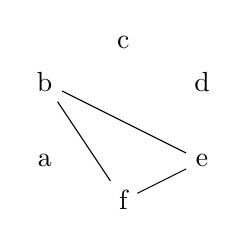
\begin{tikzpicture}
        \node(a) at (0,0) {a};
        \node(b) at (0,1) {b};
        \node(c) at (1,1.5) {c};
        \node(d) at (2,1) {d};
        \node(f) at (1, -0.5) {f};
        \node(e) at (2, 0) {e};
        \draw(b)--(e);
        \draw(b)--(f);
        \draw(f)--(e);
        \end{tikzpicture}\\
        
        17. \begin{tikzpicture}
        \node(a) at (0,0) {a};
        \node(b) at (0,1) {b};
        \node(c) at (1,1.5) {c};
        \node(d) at (2,1) {d};
        \node(f) at (1, -0.5) {f};
        \node(e) at (2, 0) {e};
        \draw(c)--(d);
        \draw(c)--(e);
        \draw(e)--(d);
        \end{tikzpicture}\\
        
        18. \begin{tikzpicture}
        \node(a) at (0,0) {a};
        \node(b) at (0,1) {b};
        \node(c) at (1,1.5) {c};
        \node(d) at (2,1) {d};
        \node(f) at (1, -0.5) {f};
        \node(e) at (2, 0) {e};
        \draw(c)--(d);
        \draw(c)--(f);
        \draw(f)--(d);
        \end{tikzpicture}\\
        
        19. \begin{tikzpicture}
        \node(a) at (0,0) {a};
        \node(b) at (0,1) {b};
        \node(c) at (1,1.5) {c};
        \node(d) at (2,1) {d};
        \node(f) at (1, -0.5) {f};
        \node(e) at (2, 0) {e};
        \draw(c)--(e);
        \draw(c)--(f);
        \draw(f)--(e);
        \end{tikzpicture}\\
        
        20. \begin{tikzpicture}
        \node(a) at (0,0) {a};
        \node(b) at (0,1) {b};
        \node(c) at (1,1.5) {c};
        \node(d) at (2,1) {d};
        \node(f) at (1, -0.5) {f};
        \node(e) at (2, 0) {e};
        \draw(d)--(e);
        \draw(d)--(f);
        \draw(f)--(e);
        \end{tikzpicture}\\
\end{document}